\documentclass[brazil]{book}
\usepackage{babel}
\usepackage[utf8x]{inputenc}
\usepackage{url}
\usepackage{graphicx}
\usepackage{html}

\title{Genos Handbook}
\author{Pedro Kröger}

\begin{document}
\graphicspath{{figs/}}

\maketitle

\begin{htmlonly}
  Baixe a versão em pdf \htmladdnormallink{aqui}
  {http://genos.mus.br/handbook/genoslab-handbook.pdf}.
\end{htmlonly}

\tableofcontents

\part{Introdução}
\label{part:introducao}

\part{Programas de áudio}
\label{part:programas-de-audio}

\chapter{CLM---Common Lisp Music}
\label{cha:clm-common-lisp}

\section{Pré-requisitos}
\label{sec:pre-requisitos}

Para compilar o CLM você precisará do gcc (o compilador C do projeto
GNU) e outras ferramentas instaladas. Além disso, o CLM não é um
programa auto-contido como o Csound. Ele é na verdade uma biblioteca
de funções Lisp. Para utiliza-lo você precisará de um compilador Lisp.
Eu recomendo o SBCL. Finalmente, você precisará de um bom editor. Eu
recomendo o Emacs com o Slime. O comando abaixo deve instalar tudo que
você precisa para começar:

\begin{verbatim}
aptitude install gcc emacs22 slime sbcl
\end{verbatim}

\section{Instalação}
\label{sec:instalacao}

Infelizmente não existe um pacote do CLM para o debian, então teremos
que instala-lo manualmente. Além disso, vamos instalar de uma maneira
que é mais fácil mas não é necessariamente robusta. Contudo essa
maneira é suficiente para você iniciar no programa. No futuro veremos
maneiras mais robustas de instalar o CLM.

Baixe a última versão do CLM no site do projeto em
\url{http://ccrma.stanford.edu/software/clm/} e descompacte o tar.gz
em um diretório. O diretório clm-3 será criado quando o arquivo for
descompactado. Os comandos abaixo efetuam essas operações:

\begin{verbatim}
wget ftp://ccrma-ftp.stanford.edu/pub/Lisp/clm-3.tar.gz
tar -xzf clm-3.tar.gz
\end{verbatim}

Observe que dentro do diretório clm-3 existem diversos arquivos. Os
arquivos com a extensão *.ins definem instrumentos do CLM e são os que
nos interessam. O próximo passo é compilar o CLM. Para isso inicie o
emacs e slime com \texttt{M-x slime}. O REPL (\textit{Read Eval Print
  Loop}) é o modo interativo de Lisp. Nele você pode digitar
expressões e obter resultados. Para programas maiores é desconfortável
entrar expressões no REPL, mas para testar coisas ele é bastante útil.
No REPL digite o comando abaixo para definir o diretório padrão. Esse
diretório deve ser onde você descompactou o CLM.

\begin{verbatim}
(setf *default-pathname-defaults* #p"/home/kroger/clm-3/")
\end{verbatim}

A figura abaixo mostra o resultado dessa expressão no emacs.

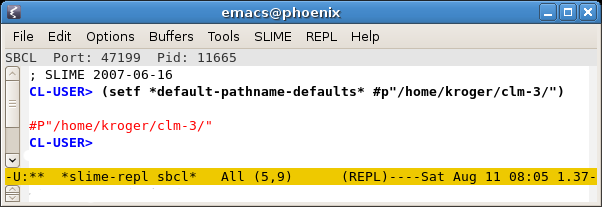
\includegraphics{slime1}

Agora rode o comando abaixo para compilar o CLM.

\begin{verbatim}
(load "all.lisp")
\end{verbatim}

\section{Uso básico}
\label{sec:uso-basico}

Tendo compilado o CLM você pode carregar e usar instrumentos definidos
nos arquivos *.ins. Por exemplo, o arquivo v.ins define um instrumento
de nome ``fm-violin'' que sintetiza um violino usando FM. Antes de
carregar os arquivos com instrumentos é necessário compilá-los. Você
pode fazer isso em uma  única etapa:

\begin{verbatim}
(load (compile-file "v.ins"))
\end{verbatim}

Contudo você só precisa compilar os instrumentos uma única vez (a
menos que o instrumento seja modificado). Se o instrumento já tiver
sido compilado, é só carrega-lo com:

\begin{verbatim}
(load "v")
\end{verbatim}

Finalmente, você pode usar o instrumento com o comando abaixo:

\begin{verbatim}
(with-sound () (fm-violin 0 1 440 .1)) 
\end{verbatim}

\section{Para saber mais}
\label{sec:para-saber-mais}

Para saber mais sobre a instalação do CLM veja o arquivo README.clm.
O manual está no arquivo clm.html. Ambos estão no diretório do CLM.

\chapter{Nyquist}
\label{cha:nyquist}

\section{Instalação}
\label{sec:instalacao-1}

Para instalar o nyquist é só usar o aptitude:

\begin{verbatim}
aptitude install nyquist
\end{verbatim}

O binário do nyquist se chama \texttt{ny}. Se você digitar \texttt{ny}
no terminal um prompt interativo vai abrir e esperar por comandos.
Você pode digitar algo simples para testar se o programa está
funcionando. O comando abaixo vai tocar um dó contral:

\begin{verbatim}
(play (osc 60))
\end{verbatim}

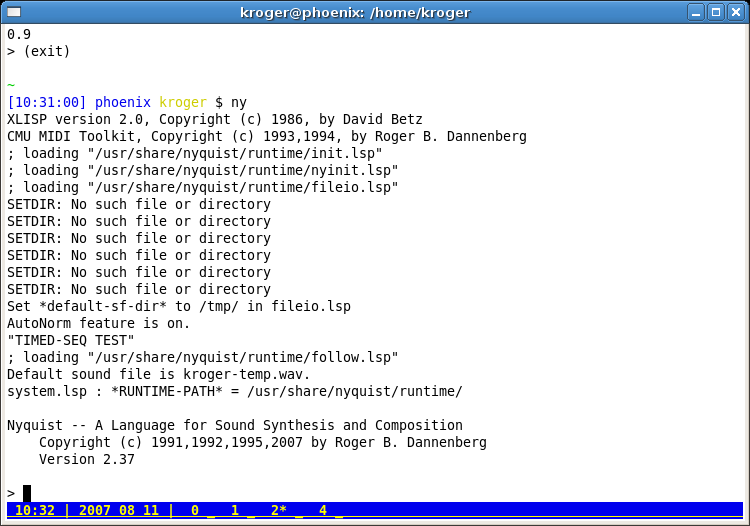
\includegraphics{ny1}

Nyquist vem com uma IDE escrita em Java. Ela ainda não está no pacote
do debian. Eu confesso que essa IDE não é muito boa. Eu prefiro
desenvolver usando o bom e velho Emacs. O problema é que não existe um
modo específico para o Nyquist, e se você configurar o emacs
globalmente para o Nyquist vai interferir com o Slime. A solução que
eu dou por enquanto é salvar \htmladdnormallink{essas
  configurações}{http://www.audacity-forum.de/download/edgar/nyquist/nyquist-doc/examples/emacs/main.html}
em um arquivo nyquist.el, carregar o emacs sem as configurações de
usuario (ou seja, sem carregar o .emacs) e carregar o arquivo
nyquist.el quando o emacs iniciar. Esse método é meio gambiarrico, mas
até ter uma solução adquada parece ser a melhor maneira.

\end{document}
